\newpage
\section*{Energy Calibration}

Before proceeding with the study of positronium decay each detector has to be energy calibrated. The $^{22}$Na source was used, considering the 511 and  1275~keV photopeaks. Calibrated spectra for each detector are presented in Fig.~\ref{Fig:Calibrated_spectra}.

\begin{figure}[h!]
	\centering
	\subfloat[][\emph{Detector 1 $^{22}$Na spectrum }.]
	{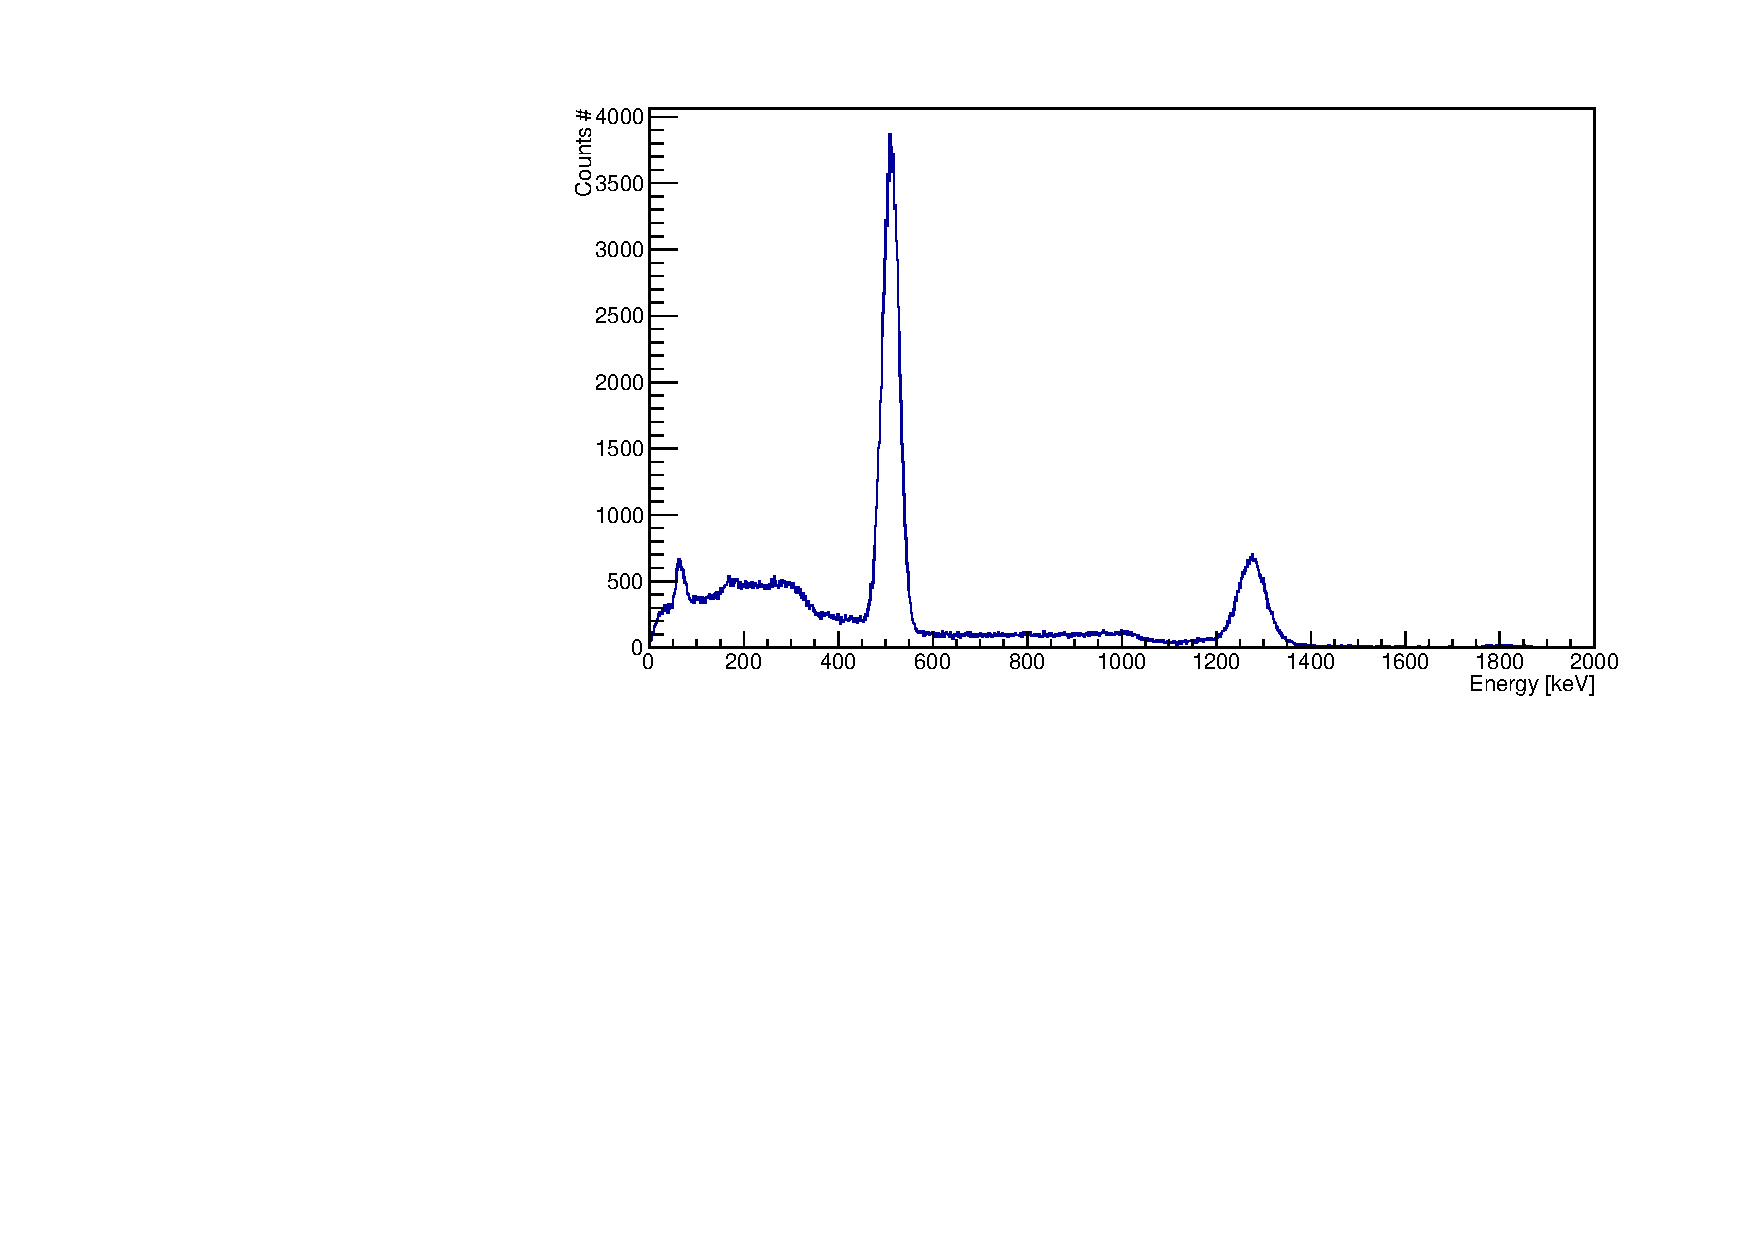
\includegraphics[width=.45\textwidth]{Det_1}} \quad
		\subfloat[][\emph{Detector 2 $^{22}$Na spectrum }.]
	{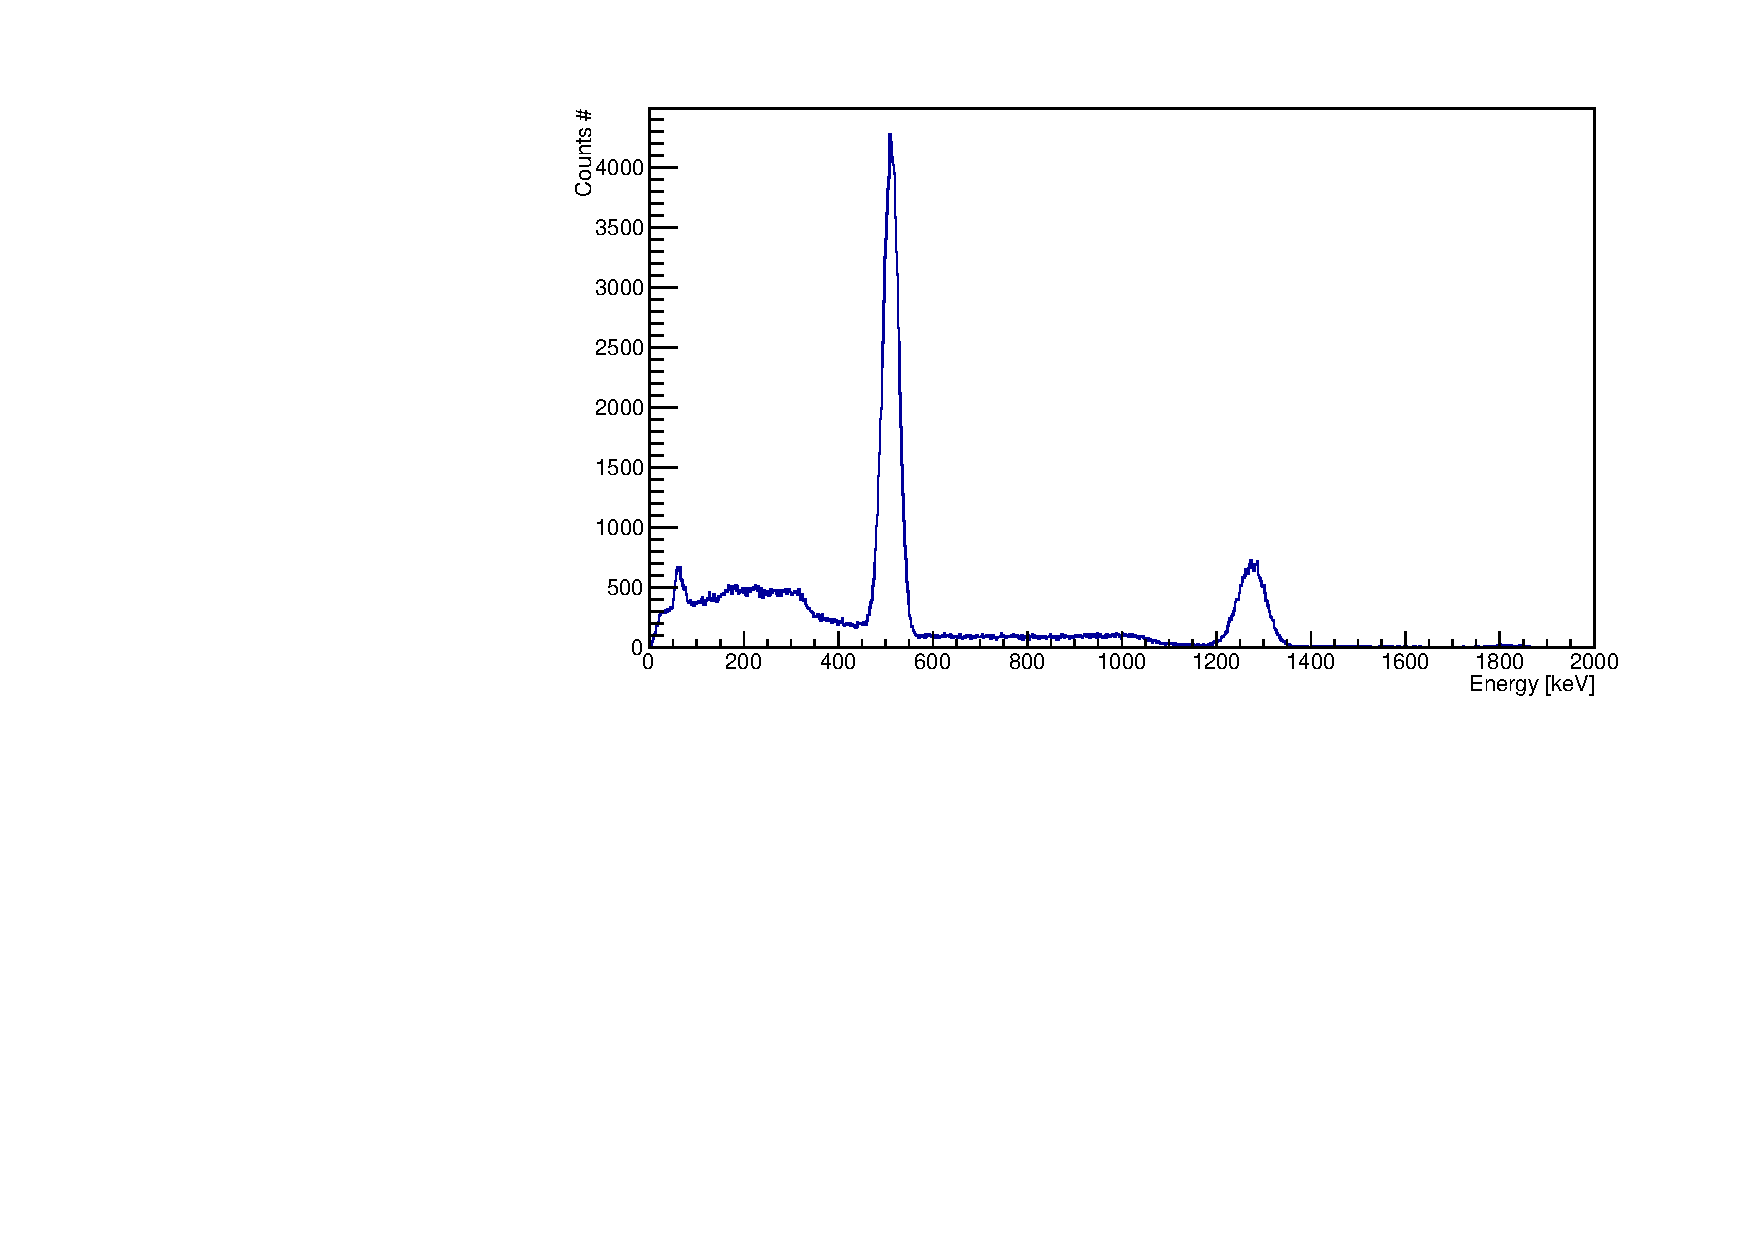
\includegraphics[width=.45\textwidth]{Det_2}} \quad 
		\subfloat[][\emph{Detector 3 $^{22}$Na spectrum }.]
	{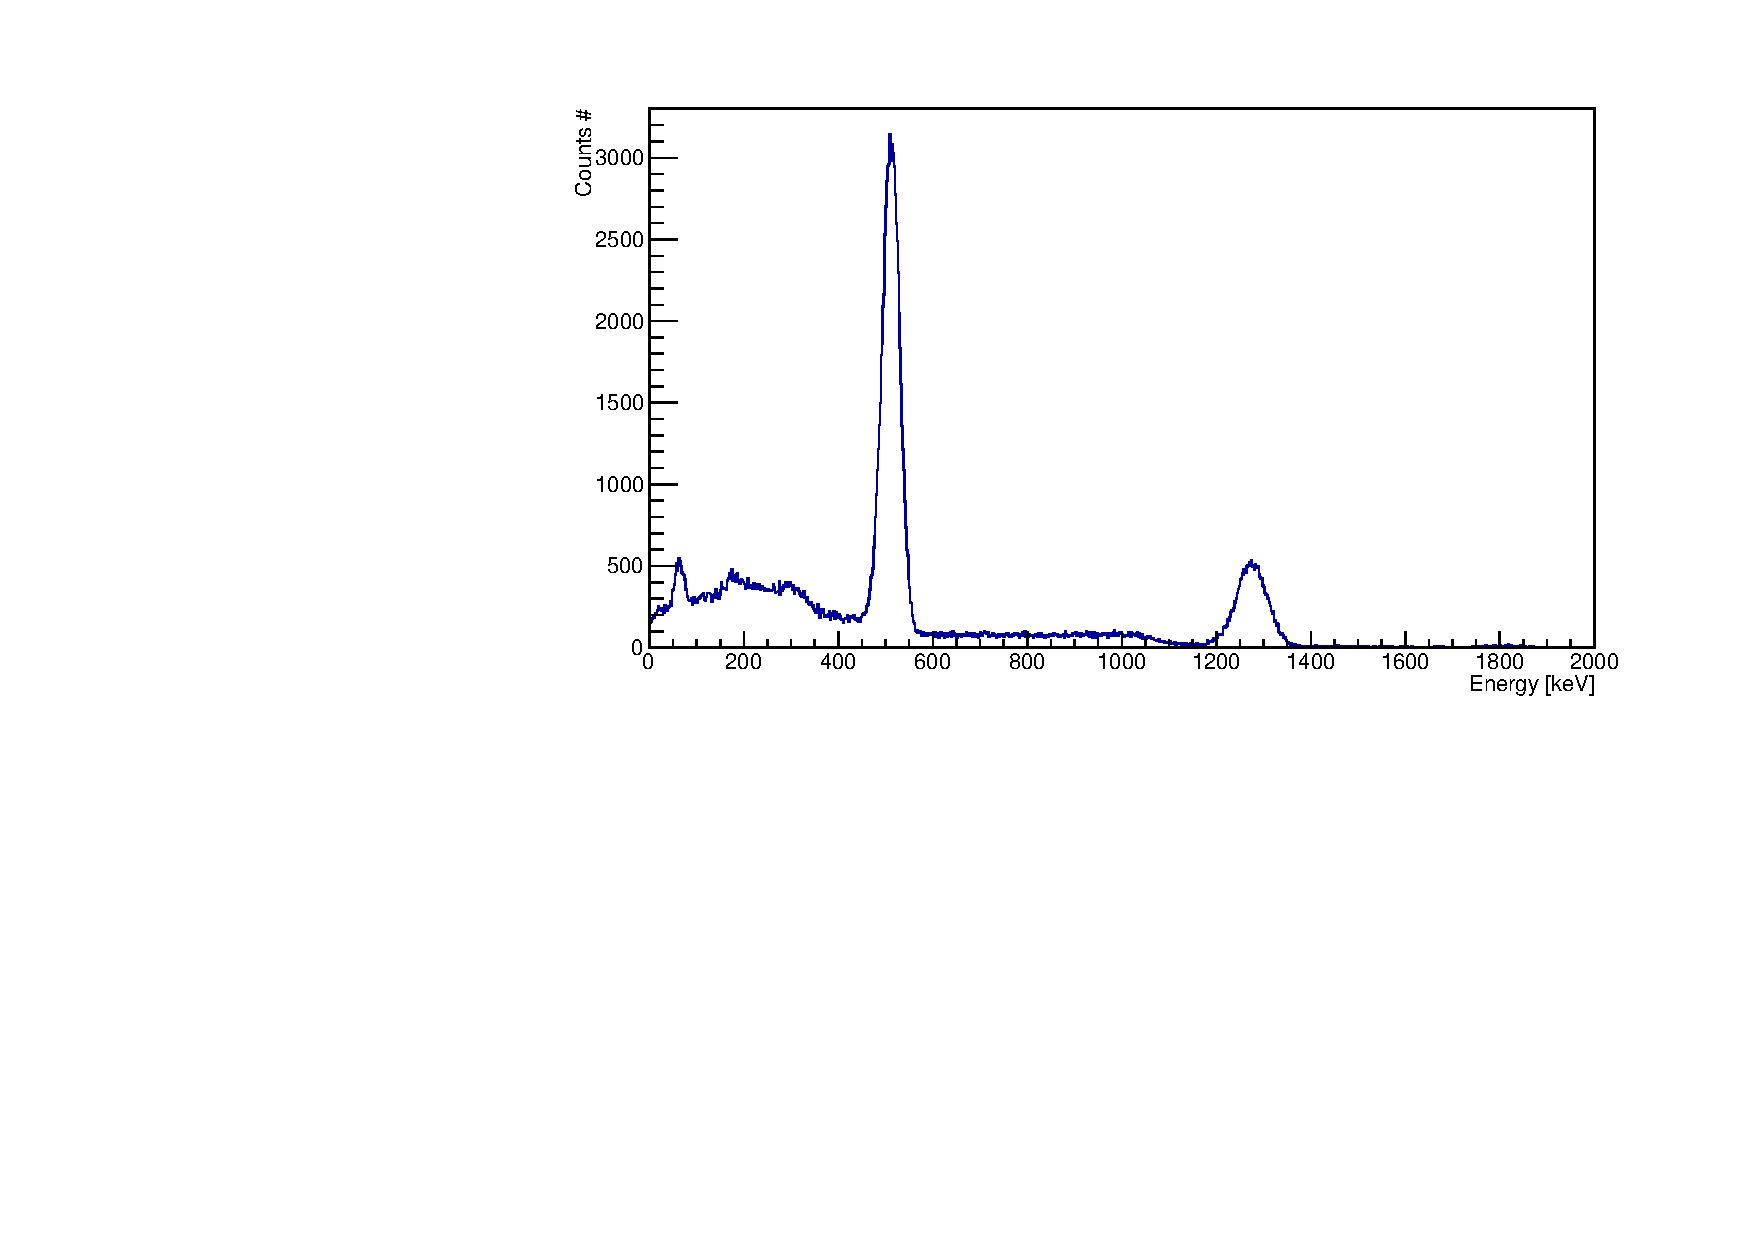
\includegraphics[width=.45\textwidth]{Det_3}} \quad
		\subfloat[][\emph{Detector 4 $^{22}$Na spectrum }.]
	{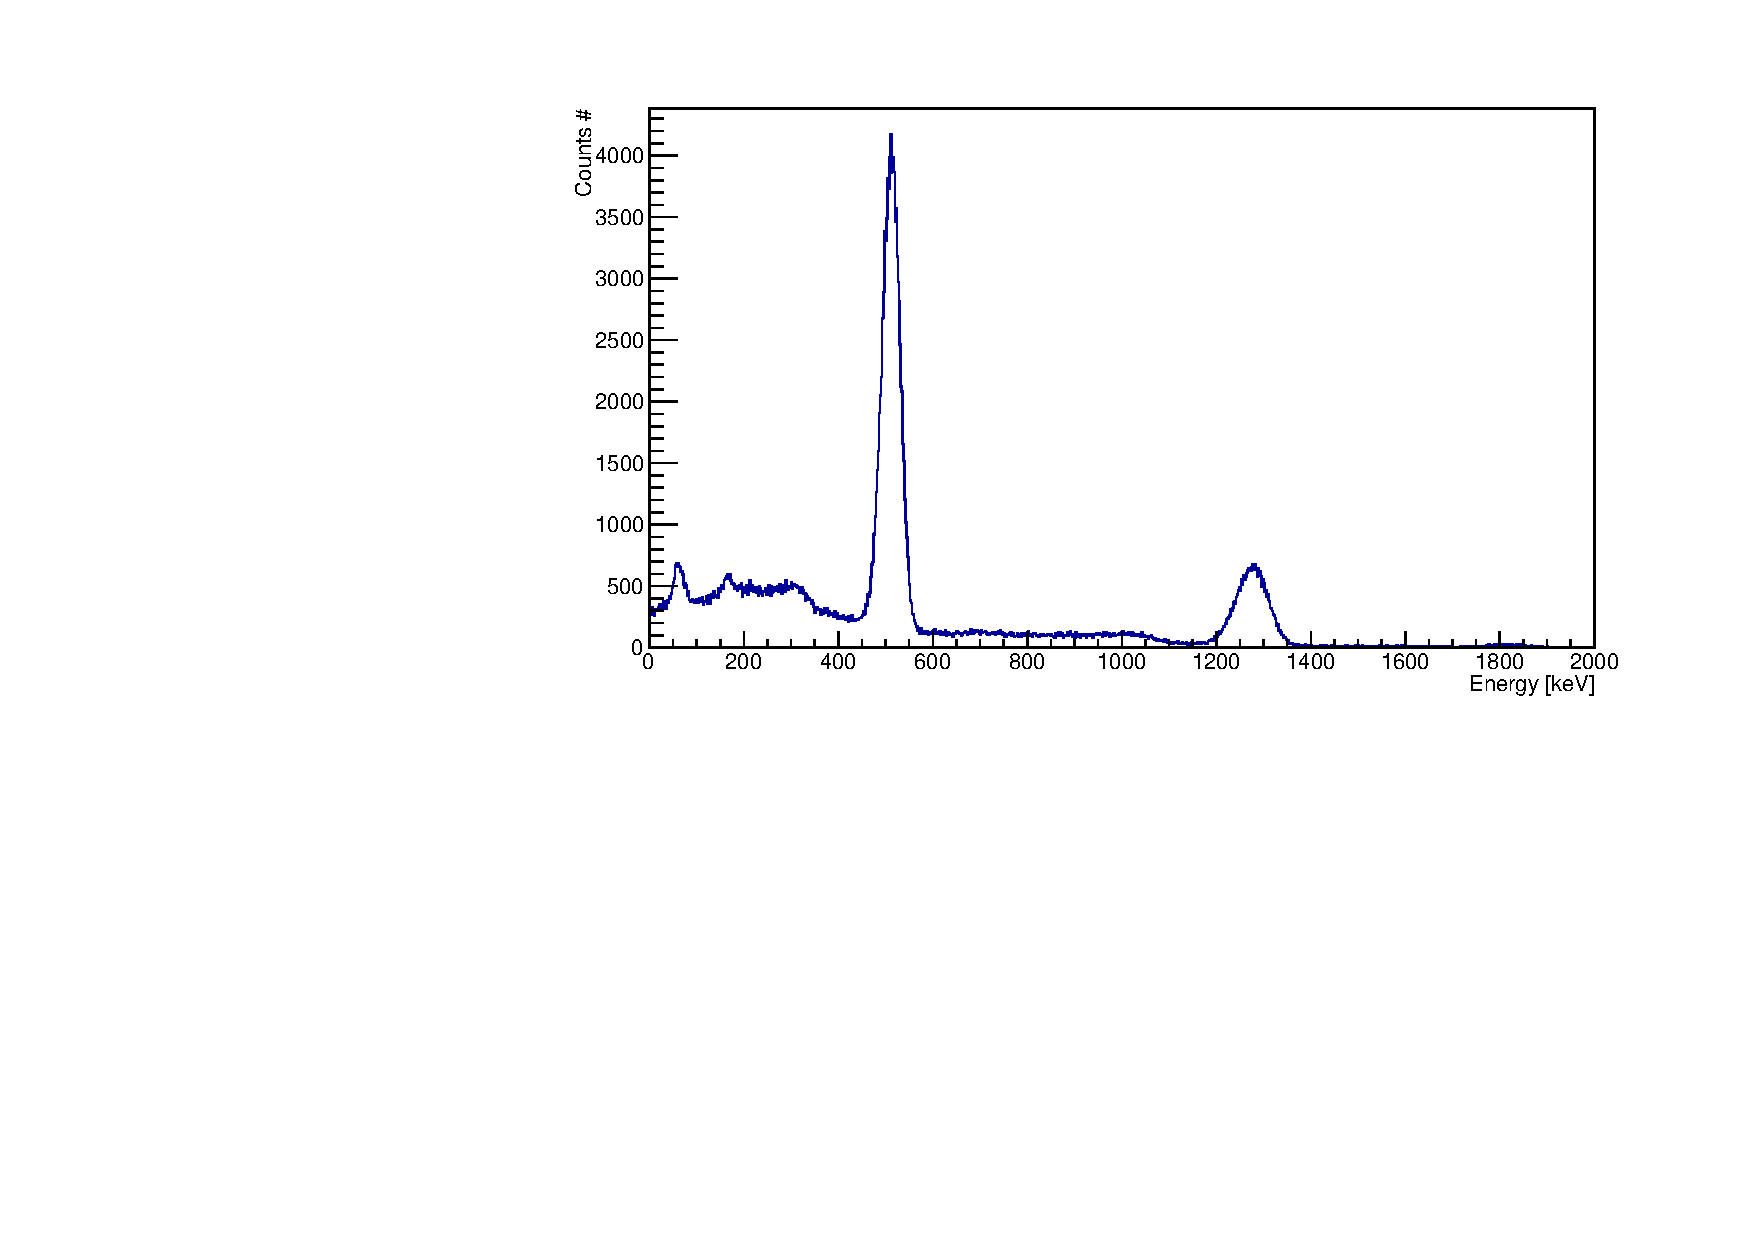
\includegraphics[width=.45\textwidth]{Det_4}} \\
	\caption{Calibrated spectra of the four detectors used in the experiment, obtained with $^{22}$Na $\gamma$-source .}
	\label{Fig:Calibrated_spectra}
\end{figure}
% Capire che errore piazzare sui parametri dei fit

\section*{TAC Calibration}

In order to calibrate the TAC unit, several spectra were produced using the autocoincidence of a detector signal delayed by a chosen
value. With 2 ns delay steps the spectrum of Fig.~\ref{Fig:Tac_calibration}-\emph{a} was obtained, the peaks
centroid were used to compute the calibration parameters performing a linear fit~(see Fig.~\ref{Fig:Tac_calibration}-\emph{b}).

\begin{figure}[H]
\centering
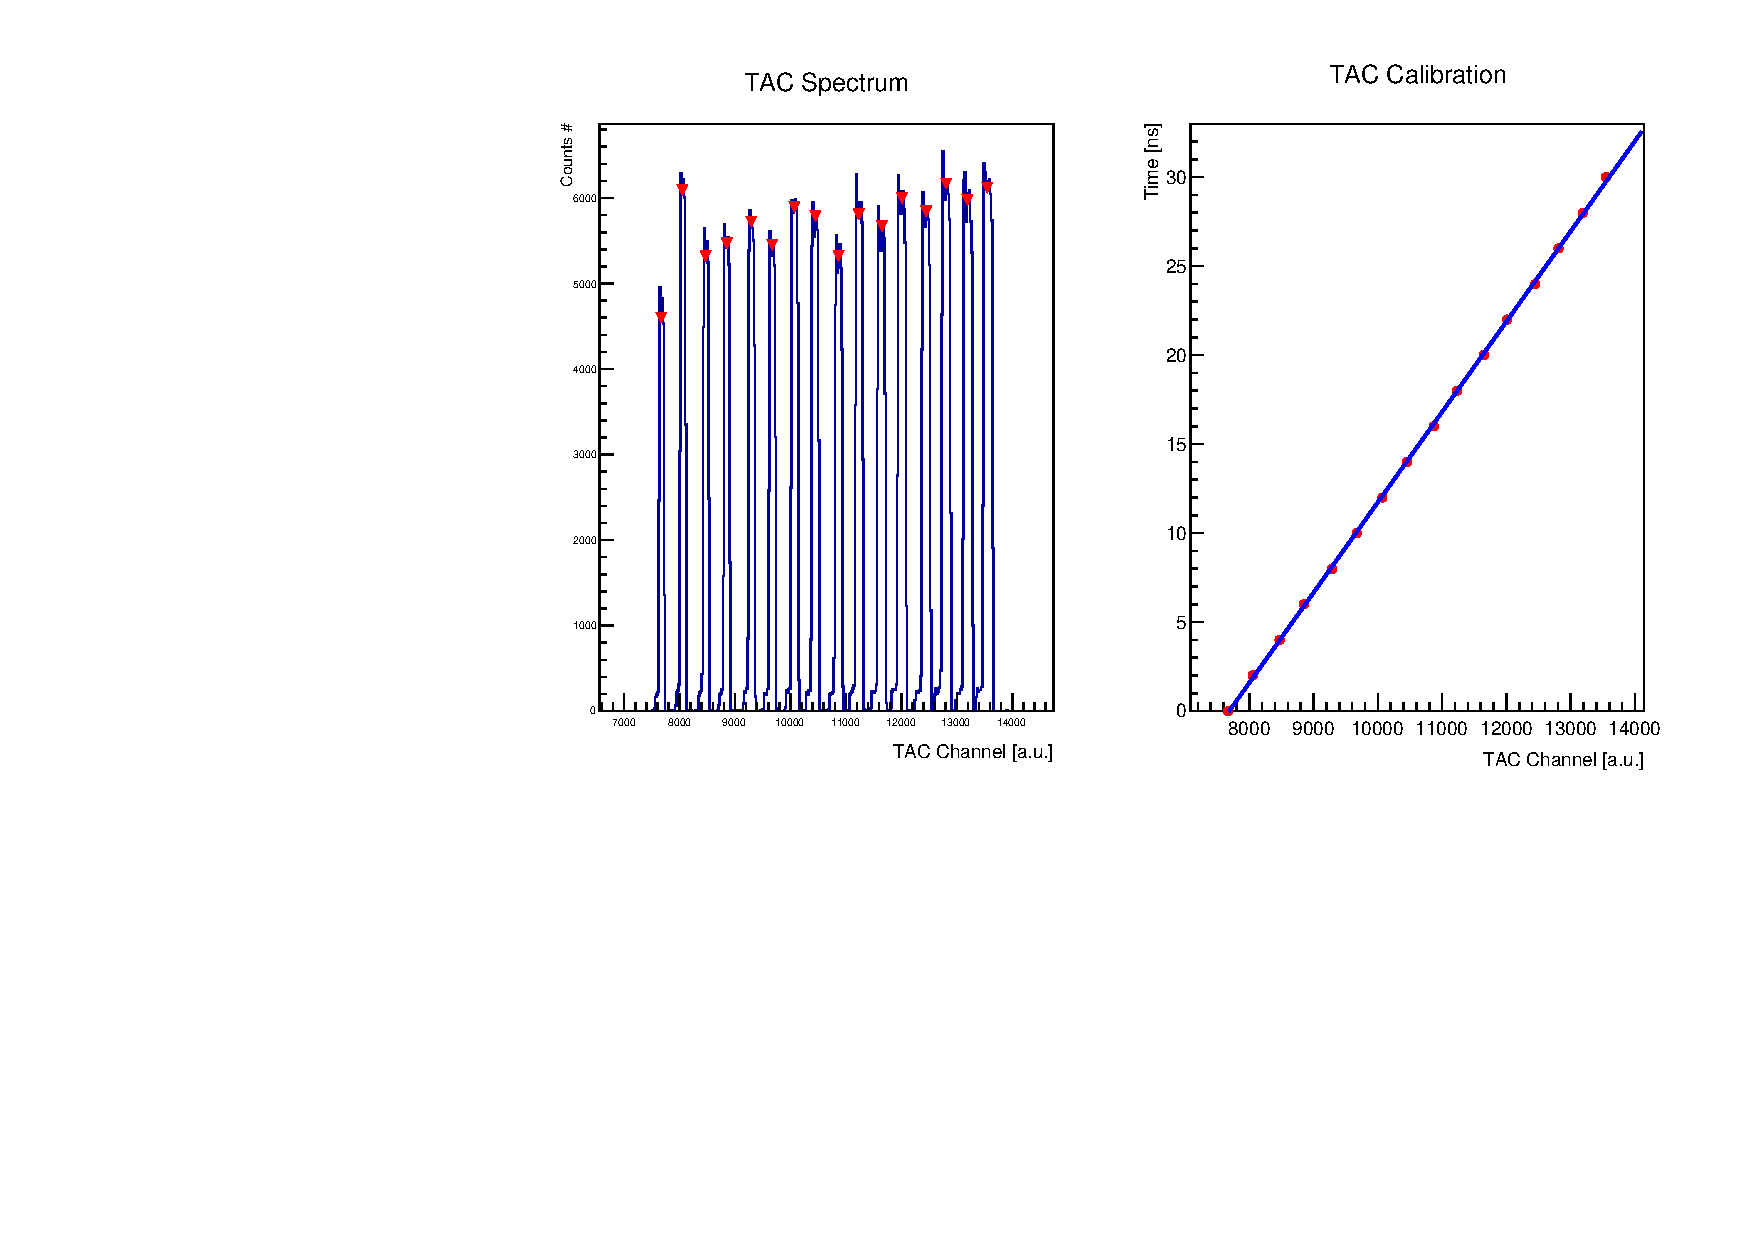
\includegraphics[width = 0.8\textwidth]{tac_cal}
\caption{Uncalibrated TAC spectrum obtained with 2~ns delay autocoincidence signals~(\emph{a}) and calibration Fit~(\emph{b}).}
\label{Fig:Tac_calibration}
\end{figure}

\begin{table}[H]
\centering
\begin{tabular}{cc}
\toprule
P0 [ns] & P1 [ns/ch] \\
\midrule
-38.9 $\pm$ 0.2 & (5.07 $\pm$ 0.02)$\times 10^{-3}$\\
\bottomrule
\end{tabular}
\caption{TAC calibration parameters.}
\label{Tab: tac calibration parameters}
\end{table}
